\chapter{Results and Future Work}\label{chapter:Conclusion}
\section{Result}
After using the Algorithm Analysis package to perform analysis on the gradient descent on classes of $m-L$ sector bounded functions where the condition number L/m are chosen between 1 and 100, the convergence rate guarantee found for each condition number is shown in Figure~\ref{plot_result}.

% \begin{code}{julia}{A sample code listing. The method \texttt{rate} performs the automated algorithm analysis by searching for a Lyapunov function that bounds the rate of convergence of the performance measure.}{code:label}
%     m,L = 1,10                                   # parameters
%     α = 2/(L+m)                                  # stepsize
    
%     @algorithm begin
%       f = DifferentiableFunctional{Rⁿ}()       # objective function
%       xs = first_order_stationary_point(f)     # first-order stationary point
%       f' ∈ SectorBounded(m, L, xs, f'(xs))     # function class
%       x0 = Rⁿ()                                # initial point
%       x1 = x0 - α*f'(x0)                       # gradient descent
%       x0 => x1                                 # state update
%       performance = (x1-xs)^2                  # performance measure
%     end
    
%     rate(performance)                            # automated algorithm analysis
%     \end{code}

\begin{figure}[h]
    \centering
    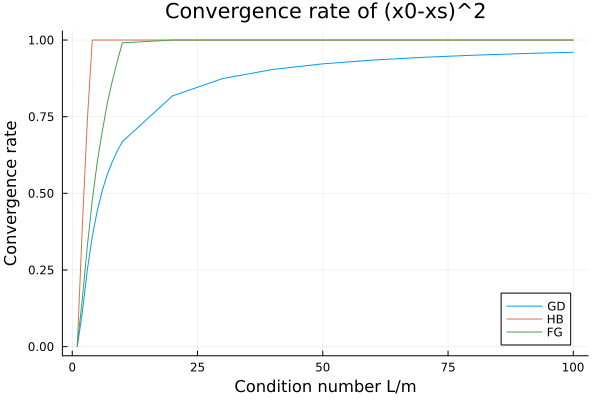
\includegraphics[width = .8 \textwidth]{plot.pdf}
    \caption{Convergence rate guarantee of gradient descent at optimizing $1-10$ sector bounded functions}
    \label{plot_result}
\end{figure}

\section{Future work}
Following this thesis proposal, the future work include finish coding the program. While most to all of the package have been coded, the program is only able to produce result correctly matching the analysis result produced in \cite{tutorial} for the gradient descent algorithm. As a result, the program need to be debugged and tested to ensure it is able to correctly implement the mathematical approach to algorithm analysis and produce accurate results.

Additionally, the program currently does not support ''lifting dimension'', an optional step of the Lyapunov method to algorithm analysis in \cite{tutorial}. Part of the future work of this research work is to implement this step and measure its effect on the tightness of the convergence rate guarantee.

A crucial step before the package can be completed and delivered as end-user software and part of the future work of this thesis is the documentation of Algorithm Analysis, which includes writing operating instructions, providinig analysis examples, detailing the package's components, and the steps the program takes to perform algorithm analysis.